\documentclass{bioinfo}
\usepackage{epstopdf}
\usepackage{url,color}
\copyrightyear{2015}
\pubyear{2015}

\usepackage{subfigure,bm,algorithm,algorithmic,color,subfigure}
\def \M {\mathcal{M}}
\def \x {\mathbf{x}}
\def \R {\mathbb{R}}
\def \D {\mathcal{D}}
\def \xh {\widehat{\x}}
\def \f {\mathbf{f}}
\def \P {\mathbf{P}}
\def \ab {\boldsymbol \alpha}
\def \X {\mathcal{X}}
\def \E {\mathrm{E}}
\def \z {\mathbf{z}}
\def \L {\mathcal{L}}

\newtheorem{thm}{Theorem}

\usepackage{citesort}
\usepackage{pslatex}
\usepackage{epsfig}
\usepackage{epsf}
\usepackage{amsmath, amsthm, amssymb, multirow, paralist, subfigure}
\usepackage{graphicx}


\begin{document}

\firstpage{1}

\title{Towards Measuring Plant Photosynthetic Heterogeneity}
\author[Tessmer \textit{et~al}]{Oliver L Tessmer\,$^{1}$, Xi Yin\,$^{1}$, Jeffrey A Cruz\,$^{2,3}$, Linda J Savage\,$^{2}$, Xiaoming Liu\,$^{1}$, David M Kramer\,$^{2,3,\ast}$, and Jin Chen\,$^{1,2,\ast}$ \footnote{to whom correspondence should be addressed}
\address{$^{1}$Department of Computer Science and Engineering, Michigan State University, East Lansing, MI 48824, USA\\
$^{2}$Department of Energy Plant Research Laboratory, Michigan State University, East Lansing, MI 48824, USA\\
$^{3}$Department of Biochemistry and Molecular Biology, Michigan State University, East Lansing, MI 48824, USA}

\history{Received on XXXXX; revised on XXXXX; accepted on XXXXX}

\editor{Associate Editor: XXXXXXX}

\maketitle

\begin{abstract}


\\
\bf{1} Department of Computer Science and Engineering, Michigan State University, East Lansing, MI, USA
\\
\bf{2} Department of Energy Plant Research Laboratory, Michigan State University, East Lansing, MI, USA
\\
\bf{3} Department of Biochemistry and Molecular Biology, Michigan State University, East Lansing, MI, USA
\\
$\ast$ E-mail: jinchen@msu.edu, kramerd8@msu.edu
\end{flushleft}

% Please keep the abstract between 250 and 300 words
\section*{Abstract}

Photosynthetic heterogeneity is a universal phenomenon among plants...

\section*{Author Summary}

Photosynthetic heterogeneity is a universal phenomenon among plants...

\section*{Introduction}


%[Phenotyping]
Using sunlight, water and $CO_2$, plants produce sugars and release $O_2$ with photosynthesis \cite{kramer2011importance}. The process involves the formation of high energy intermediates capable of generating reactive oxygen species. The photosynthetic apparatus, chloroplast and surrounding leaf tissue is inherently susceptible to oxidative damage, especially under stress conditions when the supply of light energy exceeds the capacity to utilize it \cite{asada1996radical,durrant1990characterisation}. Plants have evolved a number of mechanisms, such as photosynthetic apparatus damage and repair \cite{melis1999photosystem}, to dissipate excess light energy to minimize the potential for damage at the expense of photosynthetic efficiency \cite{adams2006energy,rochaix2014regulation}. However, these mechanisms are sensitive to leaf development and thus may change from one leave tissue to another, resulting in heterogenous photosynthetic patterns (see Figure \ref{fig:heterogeneityexample}). These patterns also vary with the position, size and growth rate of leaves, since leaves at the same node is unique in age. By integrating plant morphological and physiological features, measuring plant photosynthetic heterogeneity aids interpretation of the sophisticated photosynthesis phonemics data, particularly important for plant primary productivity estimation and modeling \cite{meng2007spatial}.

%Advanced technologies in high-throughput plant photosynthetic phenotyping (the Dynamic Environment Photosynthesis Imager, or DEPI) have been developed \cite{cruz2014depi,houle2010phenomics}. These systems generate huge amount of images of plant photosynthesis that can be used to quantify photosynthetic behavior in genetically diverse populations, leading to better understanding of the underlying mechanisms that control the photosynthetic properties \cite{fiorani2013future,rascher2011non}, enabling to measure variability in various photosynthetic parameters at high resolution across leaves.

%The model of spatial heterogeneity of the photosynthetic properties may reveal $CO_2$ intake capability, stomatal conductance and tolerance level to environmental changes of leaf tissues at different developmental stages.

%photosynthetic heterogeneity refers to a plant comprising multiple regions, a significant amount of which have different photosynthesis properties, %. %For example, under full sunlight photosynthesis usually captures at most only of available energy (bonner1962upper, von1981some, kramer2011importance).

Heterogeneity is a concept relating to the uniformity in a substance. The granularity of plant photosynthetic heterogeneity ranges from cells to tissues, leaves, and even the whole plant. While in-leaf variability in photosynthetic activity has been well-studied for the understanding of the effects of stomatal conductance \cite{Buckley1997,Cheeseman1991}, recent works show that photosynthetic capacity may decline with vertical gradient and leaf age \cite{chen2008effect,Kitajima2002}, suggesting that leaf-based photosynthetic heterogeneity is a key towards the understanding of plant photosynthesis.

The leaf heterogeneity in photosynthesis was firstly been studied  with a simulation model \cite{chen2008effect}. Due to the lack of high-throughput phenotyping technologies, the authors determined the effects of biochemical variability via the Farquhar model incorporating defined degrees of spatial variability of its parameters. The Farquhar model is a mechanistic, biochemical model widely used to describe steady-state $CO_2$ assimilation in leaves \cite{farquhar2001models,sharkey1985o2}. Spatial heterogeneity in photosynthesis was found to have an effect on the ability of the Farquhar model to accurately characterize photosynthesis at the leaf level \cite{chen2008effect}.

Recently, with the advent of advanced technologies of biomedical imaging, directly measuring heterogeneity has recently assumed new importance {\cite{cruz2014depi,tiihonen1996cerebral,wieneke1999non,wang2000}. The rapid development of lighting and imaging techniques enables real-time non-invasive monitoring of photosynthesis \cite{cruz2014depi,houle2010phenomics}, resulting in vast amount of chlorophyll fluorescence images of plants \cite{wituszynska2013multivariable}. These images can be used to quantify photosynthetic behavior in genetically diverse populations, enabling to measure variability of photosynthetic parameters at high resolution across leaves, leading to better understanding of the underlying mechanisms that control the photosynthetic properties \cite{fiorani2013future,rascher2011non}.



In order to measure leaf-based photosynthetic variability in a large-scale phenotyping experiment, in which hundreds of plants are screened simultaneously, it is required to automatically identify most of the leaves in all the plant chlorophyll fluorescence images, and then appropriately measure the variations of photosynthesis parameters across leaves.
%
The usual way of assessing whether the leaves of a plant are photosynthetically homogeneous or heterogeneous is by means of the Cochran's Q-test \cite{conover1999Practical} and the $I^2$ statistic \cite{higgins2003measuring,higgins2002quantifying}. %The process has three steps.
%
The Cochran's Q-test is computed by summing the squared deviations of each leaf's effect estimate from overall effect estimate, weighting the contribution of each leaf's effect estimate by its inverse variance \cite{conover1999Practical}.
%
The $I^2$ statistic measures the extent of true heterogeneity dividing the difference between the Cochran's Q-test value and its degree of freedom by the Q-test value \cite{higgins2003measuring,higgins2002quantifying}.
%
Due to the nature of plant, leaf-based photosynthetic heterogeneity often includes a small number of leaves. For example, there are less than ten rosette leaves of Arabidopsis thaliana (2-3 week old). Thus, the power of the traditional Cochran's Q-test and $I^2$ statistic in such circumstances is low \cite{higgins2003measuring, gavaghan2000evaluation,huedo2006assessing,ioannidis2007uncertainty}. Furthermore, leaves may have different growth rates, varying sizes, and different locations \cite{van1991insertional}, but none of them has yet been taken into the computation of heterogeneity.

%and none of them can take plant specific information, such as leaf position, into the heterogeneity measurement.

%We have developed a new leaf segmentation approach called PlantPH to identify leaves from photosynthesis images...

In this paper, we present a new computational framework called {\it Plant Photosynthesis Heterogeneity} (PlantPH) and use the tool to measure the leaf-level photosynthesis heterogeneity patterns of more than 100 Arabidopsis chloroplast mutant strains over dynamic lighting conditions, each with at least four replicates. It is followed with an outlier detection process to identify mutants with distinct heterogeneity patterns under specific subsets of the environmental conditions.
%
The mutant screen analysis reveals that ...



%---------------------------

\section*{Results}

Plant photosynthetic heterogeneity refers to a plant comprising multiple regions, many of which have different photosynthesis properties, potentially because of vastly different leaf developmental stage and tolerance level to environmental changes. By developing an efficient plant photosynthetic heterogeneity measure PlantPH and applying it on more than 100 Arabidopsis chloroplast mutant strains, we show that ...

\subsection*{Leaf-based heterogeneity measure} \label{sec:PlantPH}

%

%First of all, we have developed the leaf alignment algorithm \cite{yin2014}. This paper focus on the measure of

%Comparing with the existing heterogeneity approaches, our method is novel in the following ways:
%
%1.	PlantPH relies on a novel leaf alignment and tracking method... %, which considers plant-specific constraints including leaf shape similarity and symmetry. By taking the biological knowledge about the shapes of any possible leaf into account, we add flexibility to the model to fit to all the general leaves. Specifically, for leaf boundary identification, we develop a leaf symmetry based curve fitting model to define the initial shape of a leaf, and develop a plant layout based approach to define leaf tips and orientation, therefore defining the leaf initial position.  Note that since leaf is assumed to be symmetric, curve fitting could converge without large amount of training.
%
%2. PlantPH models heterogeneity of photosynthesis with size, position and growth rate...
%
%3. PlantPH refers to the differences between individual leaf photosynthesis and the pooled photosynthesis across all the leaves, with the weights being those used in the pooling method. With PlantPH, transient regional variation events that do not affect the whole plant photosynthesis, can be easily discovered.

%\subsubsection*{Leaf-based heterogeneity measure}

In this paper, we introduce a new leaf-based heterogeneity measurement called $PlantPH$ as follows.
%
First, let $T = \{T_{1}, T_{1}, \ldots, T_{n}\}$ be the set of effect estimates of a plant $p$ with $n$ leaves.
The effect estimate $T_{i}$ of leaf $l_i$ in plant $p$ is defined as the difference between the averaged photosynthetic values of the leaf and  the whole plant.
%
Mathematically, in each effect estimate $T_i$, let $u_i$ and $u_p$ be the averaged photosynthesis values of leaf $l_i$ and the whole plant $p$, respectively. Under the assumption of normal distribution and homoscedasticity, the effect estimate $T_i$ is the standardized mean difference \cite{hedges1998fixed}, which can be estimated by: %$T_{i} = c(l_i) (mean(l_i)-mean(p))/S(l_i,p)$ ,
%
\begin{equation}\label{eq:effectestimate}
T_{i} =  \frac{c(l_i)\left(\mu(l_i)-\mu(p)\right)}{S(l_i,p)}
\end{equation}

\noindent where $c(l_i)$ is a correction factor for the positive bias suffered by the standardized mean difference with small sample sizes, which can be estimated by $c(l_i) = 1-3/(4(|l_i|-1)-1)$ \cite{hedge1985statistical}. This adjustment will reduce the effect estimate of small leaves that only have a few pixels, and thus increase the robustness of the heterogeneity model \cite{huedo2006assessing}.
%
%According to the equation of $c(L_i, L_j)$, $c(L_i, L_j)$ is close to 1 for large leaves with many pixels, otherwise it is close to 0, down-weighing the value of heterogeneity.
%
The pooled estimate of the within-group standard deviation $S(l_i, p)$ can be computed with \cite{hedges1998fixed}:
%
\begin{equation}\label{eq:S}
S(l_i, p) = \sqrt{\frac{(|l_i|-1)std^2(l_i)+(|p|-1)std^2(p)}{|l_i|+|p|-2}}
\end{equation}

\noindent where $std^2(l_i)$ is the variance of leaf $l_i$, $std^2(p)$ is  the variance of the averaged values of all leaves in plant $p$, and $|p|$ are the total number of pixels of leaf $l_i$ and the whole plant $p$, respectively.

%The sample variance of $T_{ij}$ is estimated using Equation \ref{eq:ST} \cite{hedges1998fixed}.
%
%\begin{equation}\label{eq:ST}
%ST_{ij} = \frac{|L_i|+|L_j|}{|L_i||L_j|}+\frac{T_{ij}^2}{2(|L_i|+|L_j|)}
%\end{equation}

Then the Cochran's Q-test statistic for determining whether there is true leaf-based photosynthetic heterogeneity among the leaves is defined as:
%
\begin{equation}\label{eq:Q}
%Q=\sum_{i=1}^n \frac{\left(T_i-mean(T)\right)^2}{\tau^2}
Q=\sum_{i=1}^n w_i\left(T_i-\frac{\sum_{j=1}^n w_jT_j}{\sum_{j=1}^n w_j}\right)^2
\end{equation}

\noindent where $n$ is the total number of leaves of the plant $p$,  the right part of the equation is the weighted mean of effect estimates of all the leaves of the plant $p$, and $w_i=1/(\tau^2+\delta_i^2)$, where $\delta_i^2$ is the sampling variance of the effect estimate $T_i$, and $\tau^2$ is the between-study variance of all the effect estimates \cite{huedo2006assessing}.

To estimate $\delta_i^2$, the sampling variance of each effect estimate $T_i$, we use the photosynthetic value of every pixel in the high-resolution florescence images, in which the total number of samples of a plant is much greater than 1000. According to \cite{huedo2006assessing}, $\delta_i^2$ is close to 0. Hence, by ignoring the computation of  $\delta_i^2$ and replacing it with 0, we have:
%
\begin{equation}\label{eq:Q2}
%Q=\sum_{i=1}^n \frac{\left(T_i-mean(T)\right)^2}{\tau^2}
Q=\frac{1}{\tau^2}\sum_{i=1}^n\left(T_i-\frac{\sum_{j=1}^n T_j}{n}\right)^2
\end{equation}

Since both the between-study variance $\tau^2$ and the Q statistic represent the true heterogeneity among the distributions of the leaf-level photosynthesis, we move $\tau^2$ to the left of the equation and define a new measure called $PlantPH$:
%
\begin{equation}\label{eq:Q3}
PlantPH(f)=\sum_{i=1}^n\frac{\left(nT_if(l_i)-\sum_{j=1}^n T_jf(l_j)\right)^2}{n^3}
\end{equation}

In Equation \ref{eq:Q3}, $PlantPH(f)$ is a measure for determining whether there is true heterogeneity among all leaves of a plant. It is independent to the total number of leaves, allowing for being comparable among different plants. We take plant leaf morphology into the plant heterogeneity test by defining $f(.)$ as a function to measure the morphological properties (e.g., the area, position or growth rate) of a piece of leaf.

Specifically, in $PlantPH(area)$ we have $f(l_i)=area(l_i)$, which measures the leaf surface area \cite{boyes2001growth,tessmer2013functional}, and in $PlantPH(growth)$ we define $f(l_i)=growth\_rate(l_i)$ by adopting a three-parameter nonlinear growth model to compute both the absolute growth rate (AGR) and the relative growth rate (RGR) \cite{Richards1959,hunt1982plant,tessmer2013functional}. Moreover, in $PlantPH(position)$, we define $f(l_i)=position(l_i)$ to be 0 if $l_i$ is at the center of the plant, and 1 otherwise, in order to measure whether the leaves with a similar developmental stage have heterogeneous photosynthetic values.

 %we apply the following approach:
%\begin{enumerate}
%  \item Let $f(l_i)$ be $position(l_i)$ which returns 0 if $l_i$ is at the center of the plant, and returns 1 otherwise;
%  \item Compute $PlantPH(position)$ using Equation \ref{eq:Q3};
%  \item Since the above computation considers the plant center, we adjust $PlantPH(position)$ by
%\end{enumerate}

%%
%We estimate $\tau^2$ using the method of moments \cite{dersimonian1986meta}:
%
%\begin{equation}\label{eq:tau}
%\tau^2 = \left\{\begin{matrix}
% \frac{\widetilde{Q}-(n-1)}{\sum \widetilde{w_{i}}-\sum \widetilde{w_{i}}^2/\sum \widetilde{w_{i}}} & \widetilde{Q}>|T|+1\\
% 0 & else
%\end{matrix}\right.
%\end{equation}
%%
%\noindent where $\widetilde{Q}$ and $\widetilde{w_{i}}$ are the results of Q test of fixed effect estimate and the corresponding weight, which is computed as:	
%
%\begin{equation}\label{eq:weight}
%\widetilde{w_{i}} = \frac{1}{std^2(l_i)+c }
%\end{equation}
%
%%[Pos(L_i)\neq  Pos(L_j)] \times
%


\subsection*{PlantPH on Arabidopsis data}

In this experiment, wild type (col-0) and more than 100 Arabidopsis chloroplast mutant strains were grown side by side in a dynamic light condition for 3 days from 10 days old from seedling. A top-view fluorescence image was taken every 15 minutes during the day time, in order to observe the photosynthesis activity and the growth of the plants simultaneously. The overview of the experimental results is shown in Figure ???. In total, XXX fluorescence images were collected, preprocessed and fed to $PlantPH$. Note that the averaged leaf cell size of Arabidopsis is about $6000 \mu m^2$ \cite{gegas2014endopolyploidy} and our image resolution is 3600 pixels per squared inch. Therefore, each pixel in an image is sampled from about 1000 leaf cells.

The architecture of the whole process is shown in Figure \ref{fig:architecture}. First of all, we apply a leaf alignment and tracking method that we recently developed to identify most of the leaves from the top-view fluorescence images~\cite{xi2014tracking,yin2014}, and then compute the leaf-based photosynthesis value for every leaf. In addition, we add a leaf by drawing a small circle in the center of every plant to represent the young leaves that are difficult to identify.
%
All the pixels not contained in any leaf boundary are considered as an extra leaf. A leaf is ignored if its area is smaller than the plant center circle.
%
Next, we apply $PlantPH$ to compute the heterogeneity value for every plant at every snapshot, resulting in a heterogeneity matrix $H$. Finally, we recognize heterogeneity patterns in $H$ with an outlier detection method, and visually explore them with the L'Abbe plot \cite{song1999exploring}.

The results show ...



\subsection*{PlantPH on synthetic data}

A set of synthetic data were generated to test whether $PlantPH$ is properly designed.

\section*{Materials and Methods}

\subsection*{Data Acquisition and Preprocessing}

In the photosynthesis phenotyping experiment, hundreds of Arabidopsis thaliana plants (wild type and genetic variations with gene knockout) were grown side-by-side under three different light conditions (constant, sinusoid, fluctuate), for in total three days.
%
Top-view fluorescence images were collected every 15 minutes in order to observe the photosynthesis activity of all of the plants simultaneously. Each fluorescence image is a grey-scale image with a resolution of 1M pixels at 12-bit intensity.

To accurately capture the photosynthesis activities of plants from fluorescence images, a image segment method is applied to remove the background, identify every piece of leaf~\cite{yin2014}, measure the intensity of pixels on leaves, and finally convert the intensity values to the measure of four kinds of photosynthesis parameters.
%
The extracted measurements of photosynthesis parameters are presented in the form of multi-dimensional time-series, one dimension for every photosynthesis parameter.
%
%Figure ?? shows that the measurements of a photosynthesis parameter $\Phi_{II}$ at one time point are quite different for the leaves of the same plant  (i.e. plant no. 3-7 and 5-5).

\subsection*{Leaf alignment and tracking}

%For completeness, we introduce the leaf alignment and tracking approach...

The chlorophyll fluorescence images are false-color images, where the light intensity of every pixel is proportional to photosynthetic efficiency \cite{toet1996new} (see Figure \ref{fig:heterogeneityexample}). Differences between individual leaves with similar photosynthetic efficiency can be subtle, making the boundaries between them difficult to define and creating a significant challenge for subsequent shape analysis. The difficulty even arises when individual leaves overlap and occlude one another in these false-color images.

We have developed a framework based on the well-known Chamfer Matching algorithm \cite{yin2014}. Multi-leaf alignment aims to segment all leaves with pre-defined leaf templates and estimate the two tip points of each leaf. The tracking algorithm consists of two steps. First, a set of leaf templates are applied to the target image to generate the same amount of leaf candidates. Second, we adopt multi-objective optimization to select a subset of leaf candidates. The objective is to select a minimal number of leaf candidates with smaller Chamfer distances to cover the test image mask as much as possible.

Multi-leaf tracking is an extension of the leaf alignment algorithm. Given a serial of fluorescence images  taken over time, we first apply the alignment algorithm to the last frame, and then continuously apply template transformation to the current leaf candidates in order to fit to the previous frame. A new objective function considering the Chamfer Matching distances, target image mask, and the rotation angels of all leaves is adopted.
%
Both the leaf alignment and leaf tracking directly benefit the study of leaf behavior in plant biology, such as leaf growth, leaf-level photosynthesis, leaf-level variations in plant mutant, etc.

\subsection*{Heterogeneity test}

Cochran's Q-test is the classical measure of heterogeneity \cite{conover1999Practical}. In leaf-based photosynthetic heterogeneity, Q is calculated as the weighted sum of squared differences between the photosynthesis value of a individual leaf and the pooled photosynthesis value across all leaves with the weights being those used in the pooling method. The distribution of Q is a chi-square statistic with $k-1$ degrees of freedom, where $k$ is the number of leaves. Cochran's Q-test has been widely used in biomedical studies. For example, heterogeneity in the aggressiveness of tumor cell populations has been adopted as an essential feature in predicting treatment success \cite{OSullivan2003}. However, due to the nature of plant, leaf-based photosynthetic heterogeneity often includes a small number of leaves, and thus the power of the Q-test in such circumstances is low \cite{higgins2003measuring, gavaghan2000evaluation}.
%
%Conversely, Q has too much power as a test of heterogeneity if the number of leaves is large \cite{higgins2003measuring}.

%An additional test is provided with the odds ratio meta-analysis \cite{breslow1987statistical}. It is arguably not possible to examine the null hypothesis that all studies are evaluating the same effect, by considering the only the summary data from the studies: The heterogeneity test results should be considered alongside a qualitative assessment of the combinability of studies in a systematic review.

The $I^2$ statistic describes the percentage of variation across studies that is due to heterogeneity rather than chance \cite{higgins2002quantifying,higgins2003measuring}. $I^2$ can be calculated  as $I^2 = (Q - df)/Q$, where Q is Cochran's Q-test heterogeneity statistic and $df$ is the degrees of freedom. A negative value  indicates no observed heterogeneity, and larger values show increasing heterogeneity. $I^2$ is an intuitive and simple expression of the inconsistency. $I^2$ of leaf-based photosynthetic heterogeneity does not inherently depend upon the number of leaves, so that $I^2$ values of different plants become comparable. A confidence interval for $I^2$ is constructed using either the iterative non-central chi-squared distribution method \cite{hedges2001power} or the test-based method \cite{higgins2002quantifying}.

Based on Cochran's Q-test and the $I^2$ statistic, we develop a new approach that quantifies the effect of heterogeneity of photosynthesis across leaves of the same plant, and compare the degree of inconsistency among mutant strains in varying environmental conditions. The challenges of this work include the leaf alignment and the new heterogeneity measure that takes leaf position, size and growth into consideration.

%To measure leaf-based photosynthetic variability in a large-scale phenotyping experiment, in which hundreds of plants are monitored in real time, it is naturally required to identify each leaf from top-view photosynthesis images automatically. However, leaf identification is a difficult task, in that 1) all the leaves are very similar in appearance especially for model plant Arabidopsis; 2) leaf features are much fewer than the well-studied face recognition problem; and 3) leaves may overlapped with each other that makes the problem more complicated. In short, there are two challenging computational problems. First, how to separate overlapped leaves in photosynthesis images where the leaf boundaries are obscure. Second, how to recognize incomplete leafs due to occlusion. Alternatively, approximation approaches can be used to estimate the leaf-based photosynthetic heterogeneity, including distribution based, region based and pixel based approaches. While these approximation approaches are easier to model, their performance may be reduced.

% Results and Discussion can be combined.

\subsection*{Outlier detection}

%Three outlier detection methods were adopted to...

An outlier is an observation that appears to deviate markedly from other observations in the sample. Hampel (Hampel, 1971; Hampel, 1974) introduced the concept of the break-down point, as a measure for the robustness of an estimator against outliers.
%
The breakdown point is defined as the smallest percentage of outliers that can cause an estimator to take arbitrary large values. Thus, the larger breakdown point an estimator has, the more robust it is. For example, the sample mean has a breakdown point of 1/n, since a single large observation can make the sample mean and variance cross any bound.
%
Accordingly, Hampel suggested the median and the median absolute deviation (MAD) as robust estimates of the
location and the spread. The Hampel identifier is often found to be practically very effective (Perarson, 2002; Liu et al., 2004).




\section*{Discussion}

A consensus view of the data is that the photosynthesis ability of a plant is not uniform across the whole area (Charles 2008, Meng 2007).
%
The photosynthetic properties of plants can vary dramatically across cells, tissues, and organs~\cite{}, reflecting differences in development, stress responses, regulation of processes such as stomatal conductance~\cite{}, photodamage~\cite{}, and storage of photosynthate~\cite{} and contribute substantially to productivity~\cite{}.

For example, we observed that the acclimation of photosynthesis in response to cold temperatures appears to be more rapid and robust in younger or emerging than older leaves, and ecotypes isolated from different latitudes show distinct heterogeneity patterns, implying that these responses are important for adaptation of photosynthesis to fluctuating temperatures.
%
In other cases, exposure of plants to fluctuating light resulted in loss of photosynthetic capacity or increased photoinhibition in specific sets of leaves or leaf sectors. In many cases, older leaves are preferentially affected, suggesting that resources for maintenance or acclimation responses are preferentially directed to younger leaves. However, we have also identified mutant lines where younger leaves are preferentially affected, which presumably affect the development of photosynthetic robustness.

In order to systematically study the leaf level photosynthesis phenotypes, especially in a high-throughput screen manner, we developed a novel computational tool to automatically conduct statistical analysis on leaf based photosynthesis.

\section*{Acknowledgments}
This research was supported by Chemical Sciences, Geosciences and Biosciences Division, Office of Basic Energy Sciences, Office of Science, U.S. Department of Energy (award number DE-FG02-91ER20021) to JC and DMK.

\section*{References}

% Either type in your references using
% \begin{thebibliography}{}
% \bibitem{}
% Text
% \end{thebibliography}
%
% OR
%
% Compile your BiBTeX database using our plos2009.bst
% style file and paste the contents of your .bbl file
% here.
%

\section*{Figure Legends}
% This section is for figure legends only, do not include
% graphics in your manuscript file.
%
%\begin{figure}
%\caption{
%{\bf Bold the first sentence.}  Rest of figure caption.
%}
%\label{Figure_label}
%\end{figure}

\begin{figure}[!h]
%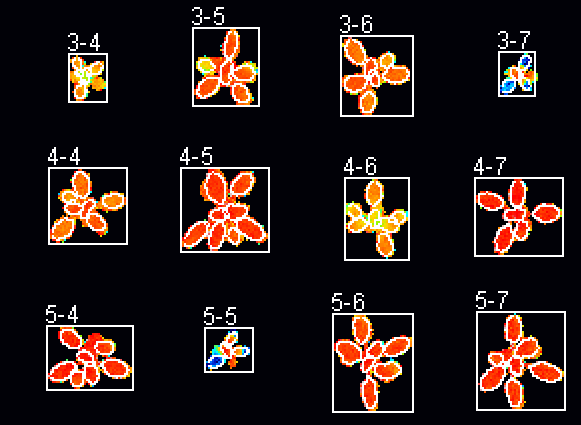
\includegraphics[width=2in]{preprocessing.png}
\caption{ Examples of leaf-level photosynthetic heterogeneity. Examples of leaf-level photosynthetic heterogeneity. Examples of leaf-level photosynthetic heterogeneity.}
\label{fig:heterogeneityexample}
\end{figure}

\begin{figure}[!h]
%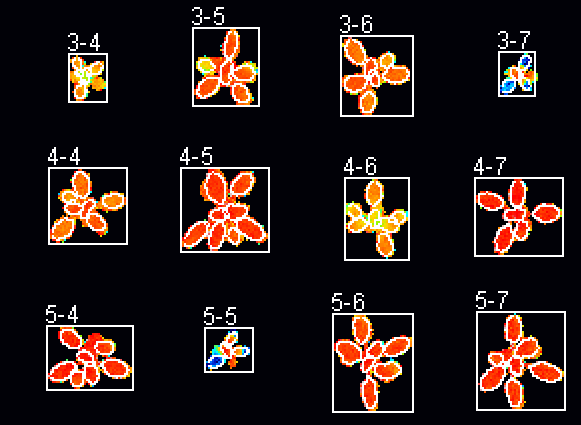
\includegraphics[width=2in]{preprocessing.png}
\caption{ The architecture of the PlantPH measurement. First, we apply a leaf alignment and tracking method that we recently developed to identify most of the leaves from the top-view fluorescence images. Second, we compute the leaf-based photosynthesis value for every leaf. Third, we apply $PlantPH$ to compute the heterogeneity value for every plant at every snapshot, resulting in a heterogeneity matrix $H$. Finally, we recognize heterogeneity patterns in $H$ with an outlier detection method, and visually explore them with the L'Abbe plot.}
\label{fig:architecture}
\end{figure}



\section*{Tables}
%
% See introductory notes if you wish to include sideways tables.
%
% NOTE: Please look over our table guidelines at http://www.plosone.org/static/figureGuidelines#tables to make sure that your tables meet our requirements. Certain types of spacing, cell merging, and other formatting tricks may have unintended results and will be returned for revision.
%
\begin{table}[!h]
\caption{Please look over our table guidelines  to make sure that your tables meet our requirements.}
\begin{tabular}{|c|c|c|}
table information
\end{tabular}
\begin{flushleft}Table caption
\end{flushleft}
\label{tab:label}
 \end{table}

\section*{Supporting Information Legends}
%
% Please enter your Supporting Information captions below in the following format:
%\item{\bf Figure SX. Enter mandatory title here.} Enter optional descriptive information here.
%
\begin{description}
\item {\bf} A
\item {\bf} B
\end{description}

\small
\bibliographystyle{plain}
\bibliography{heterogeneity}

\end{document}

